\chapter{METHODOLOGY}

This chapter describes the methodology behind the proposed therapist-led virtual group therapy system. The system is not a free-form multi-agent chatroom. It is a structured supportive dialogue engine in which the therapist remains the main user-facing voice, while the virtual group layer contributes controlled peer support only when it is useful, stage-compatible, and safe. The chapter first gives an overview of the full architecture, then explains the therapist core, blackboard coordination, Yalom-inspired peer support, and the safety and evaluation trace.

\section{Design Goals}

The proposed system is designed as a therapist-led virtual group therapy prototype. Its purpose is not to simulate an unrestricted group chat, but to combine structured therapeutic progression with carefully controlled peer support. In a typical session, the student either completes the initial screening or begins by describing a current difficulty. The therapist voice then guides the main direction of support, while Nam and Linh may add short peer-like messages only when they help the student feel less isolated, more understood, or more hopeful. Safety checks remain active throughout the process. Figure~\ref{fig:system_architecture} provides an overview of this design.

\begin{figure}[H]
\centering
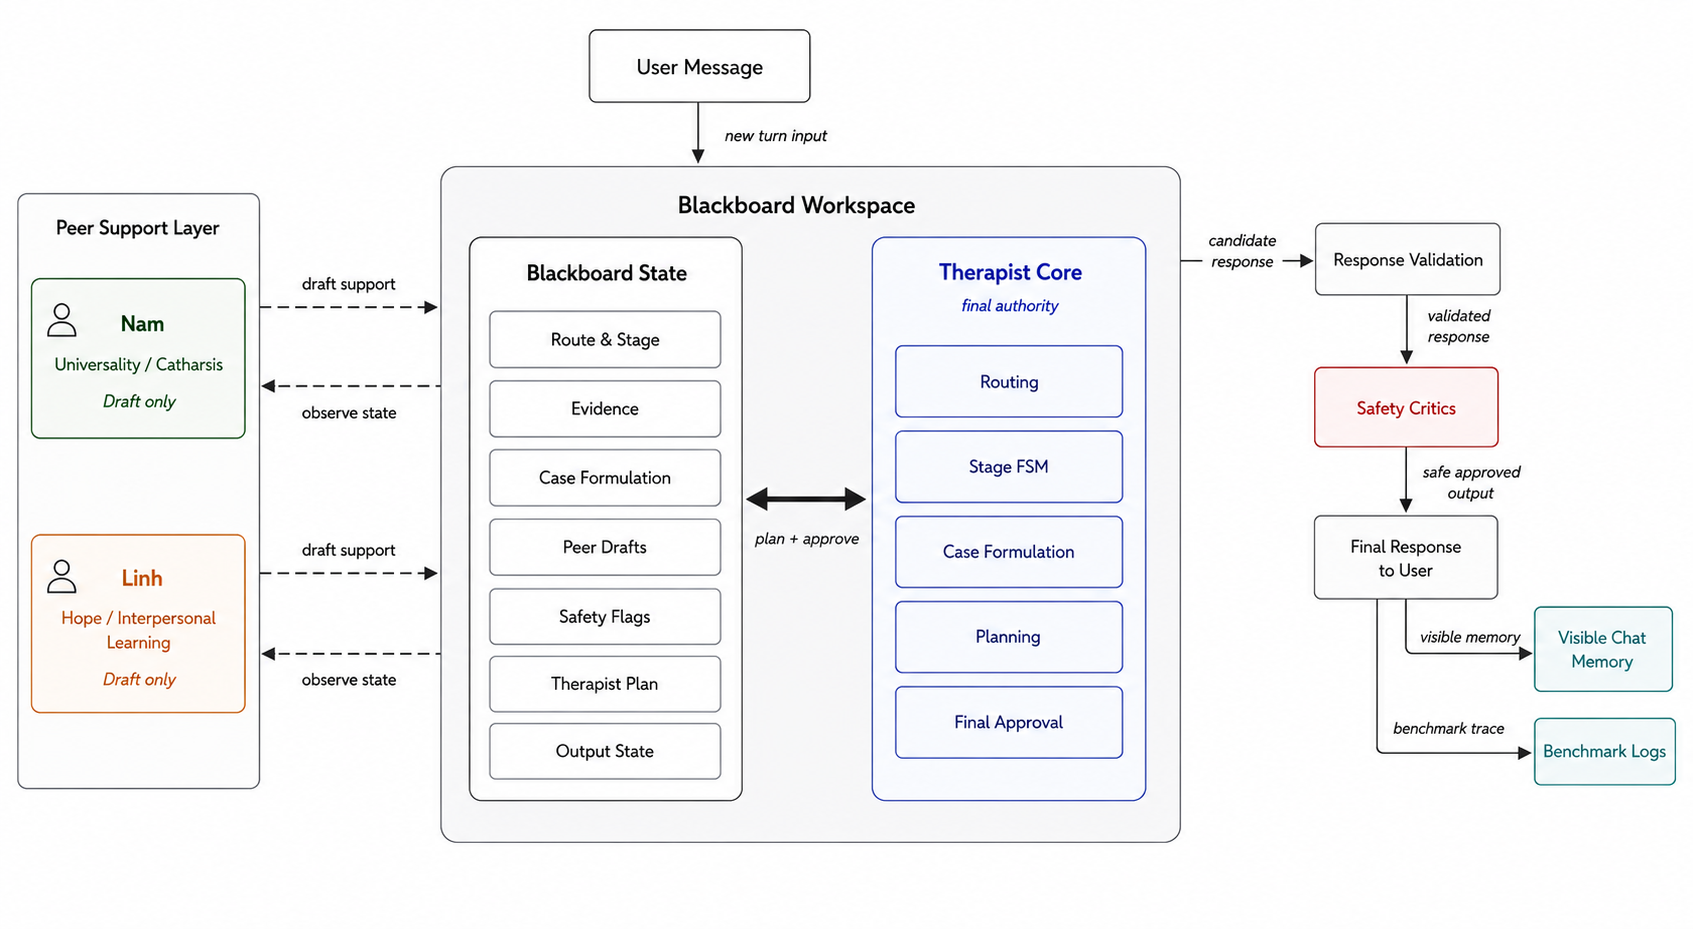
\includegraphics[width=\textwidth]{figures/fig_3_1_system_architecture.png}
\caption{Therapist-led virtual group therapy architecture.}
\label{fig:system_architecture}
\end{figure}

As shown in Figure~\ref{fig:system_architecture}, the system is organized around a shared therapeutic context. This context stores the current route, stage, safety state, peer drafts, and therapist plan. The therapist core reads and updates this context, but it remains the only component that can approve the final response. Nam and Linh observe the same context and write draft support only when their Yalom-inspired roles are relevant.

This perspective led to the following design goals:

\begin{enumerate}
    \item \textbf{Group Presence.} The system should provide a sense of being supported in a small therapeutic group rather than receiving a single generic reply. The therapist remains the main facilitator, while peer voices add a limited sense of shared experience.
    \item \textbf{Guided Progression.} The conversation should move through appropriate therapeutic stages, so that emotional support, reflection, grounding, and action planning appear at the right time. This prevents the session from becoming only repeated reassurance or premature advice.
    \item \textbf{Safe Peer Participation.} Peer voices should contribute only when they strengthen universality, catharsis, hope, or interpersonal learning, while the therapist remains responsible for the session. Silence is also treated as a valid peer behavior when a peer message would interrupt safety, grounding, or focused therapeutic work.
\end{enumerate}

To achieve the outlined goals, the system is designed with the following features:

\begin{enumerate}
    \item \textbf{Shared therapeutic context.} The system maintains a common session state so that the therapist and peer layer can respond to the same understanding of the user's route, stage, emotional need, and safety condition.
    \item \textbf{Therapist facilitation.} The therapist core guides the session, selects the next therapeutic move, and approves the final user-facing response.
    \item \textbf{Peer role boundaries.} Nam and Linh can observe the session and propose short supportive contributions, but they cannot lead the therapy or publish messages without therapist approval.
    \item \textbf{Safety and traceability.} Candidate responses pass through validation and safety checks before becoming visible, while internal decisions are kept available for later evaluation.
\end{enumerate}

The following sections unpack these features, beginning with the therapist core.

\section{Therapist Core}

The therapist core is the main layer of the system. It is designed to behave like a careful one-to-one supportive therapist before the group layer is considered. In a normal turn, the therapist speaks directly to the user, integrates any approved peer material, and remains accountable for the final response. This role is intentionally stronger than a generic empathy prompt: it must validate emotion, select a route, follow the current stage, choose one technique, avoid unsafe claims, and keep the conversation focused.

The therapist is not presented as a licensed clinician and does not provide diagnosis or treatment. This thesis treats the system as a supportive research prototype. The therapist voice is therefore designed to be warm, concise, culturally aware for Vietnamese students, and careful about uncertainty.

\subsection{Clinical Intake and Routing}

The onboarding module uses DASS-21 as an initial screening signal. DASS-21 is used only to guide routing, not to diagnose the user. By treating DASS strictly as a symptom scale rather than a diagnostic interview \citep{Lovibond1995DASS,Le2017DASS21Vietnamese}, the system can safely initialize the likely support route and determine the level of caution needed in early turns.

\subsubsection{Route Selection}

After onboarding, the system selects one of three ordinary support routes: CBT, MBI, or BA. The route is not locked forever by the initial questionnaire. The system also reads the latest user message and recent history. CBT is appropriate when the main issue involves interpretation, self-talk, or cognitive distortion. MBI is preferred when the user is overwhelmed, physiologically activated, or fused with repetitive thoughts. BA is preferred when the user shows low energy, avoidance, shutdown, or difficulty starting action.

\subsubsection{Crisis Bypass}

A separate crisis route overrides ordinary support when acute risk is detected. In that case, the system does not continue normal route selection or peer contribution. It prioritizes a direct safety-focused response and defers ordinary therapeutic progression. The detailed safety behavior is described again in Section~\ref{sec:psychosocial_safety}, where crisis handling is placed inside the broader safety pipeline.

\subsection{Evidence-Gated Stage Control}

\subsubsection{Evidence Extraction}

The clinical assessor does not simply ask the LLM to choose a stage. For CBT, the LLM is used as an evidence extractor: it identifies observable signals such as emotion, event context, automatic thought, distortion candidates, insight, balanced reframe, action step, overload, and hope request. The deterministic FSM then decides the stage from that evidence, significantly reducing the chance that the language model jumps directly to a later technique without sufficient conversational support.

For MBI and BA, the current implementation uses route-specific evidence heuristics. MBI evidence focuses on physiological activation, decentering language, body sensation, and readiness for mindful action. BA evidence focuses on energy level, avoidance, micro-action selection, scheduling barriers, and completion signals. If the CBT evidence extractor returns malformed JSON or schema-drifted fields, the system normalizes the output and falls back to heuristic evidence extraction when necessary.

\begin{table}[tb]
\centering
\caption{Evidence extraction and repair strategy.}
\label{tab:evidence_strategy}
\small
\begin{tabular}{p{0.16\textwidth}p{0.32\textwidth}p{0.34\textwidth}}
\toprule
Route & Evidence source & Repair and fallback \\
\midrule
CBT & LLM evidence extraction plus heuristic sanitizer & Normalize schema drift, reject unsupported inference, then fallback to heuristic extraction \\
MBI & Heuristic evidence from message and recent history & Use grounding, decentering, body, and mindful-action cues \\
BA & Heuristic evidence from message and recent history & Use energy, micro-action, barrier, schedule, and completion cues \\
CRISIS & Crisis and safety pattern detection & Bypass ordinary route and peer layer \\
\bottomrule
\end{tabular}
\end{table}

\begin{figure}[tb]
\centering
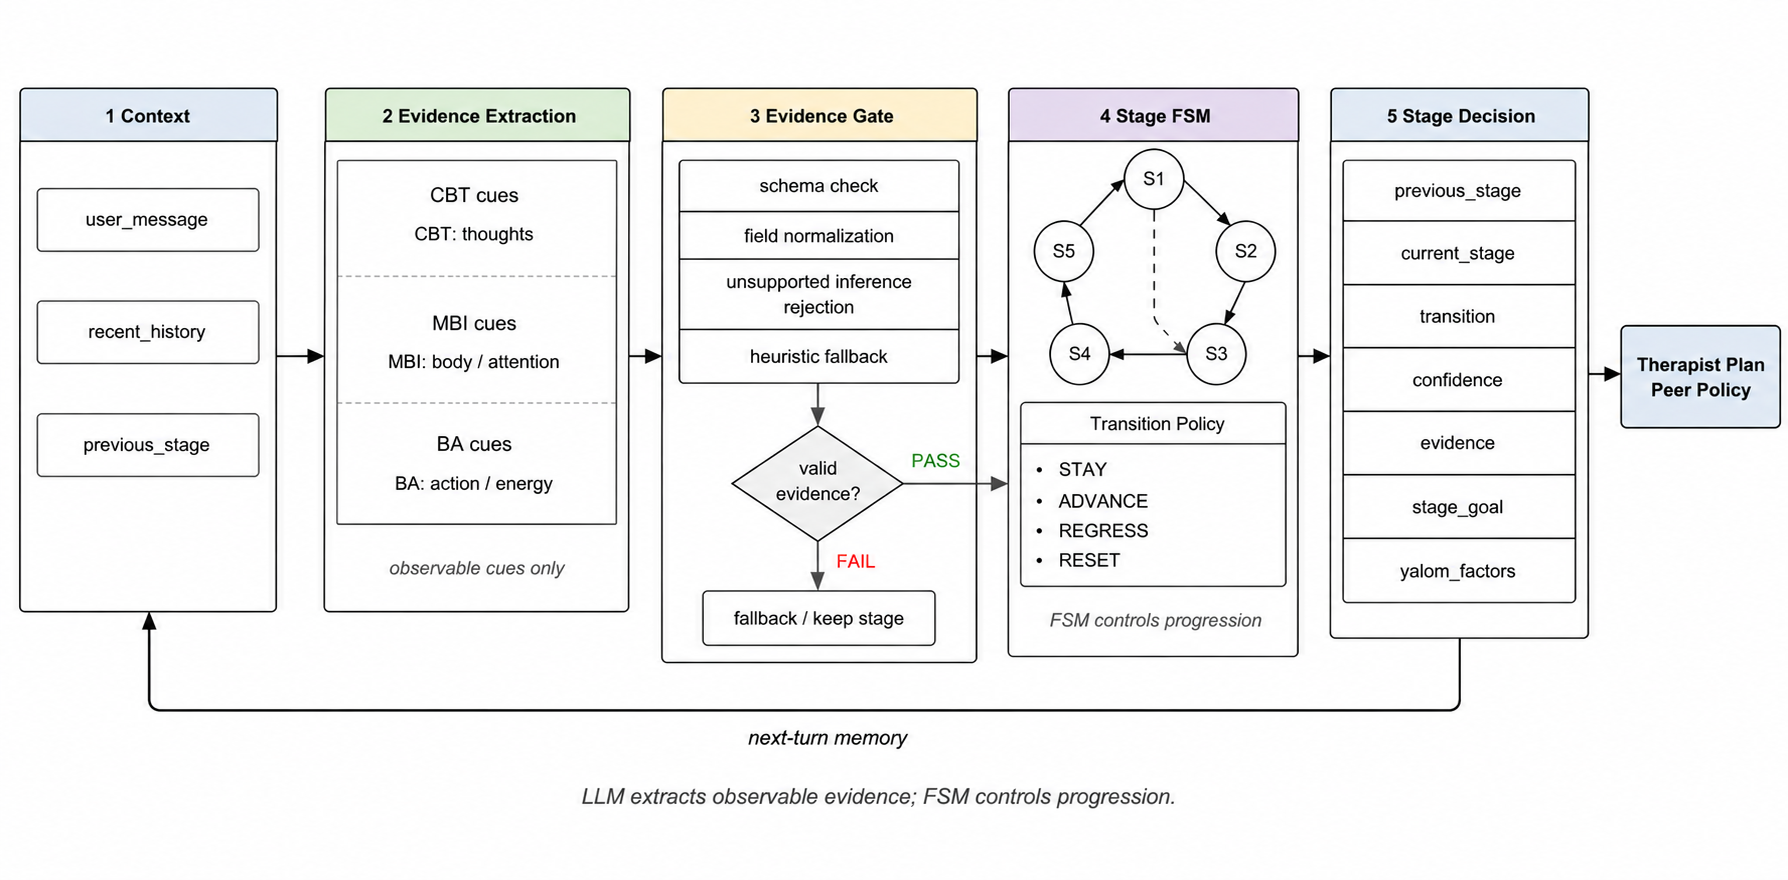
\includegraphics[width=\textwidth]{figures/fig_3_2_evidence_fsm.png}
\caption{Evidence extraction and stage FSM pipeline.}
\label{fig:evidence_fsm}
\end{figure}

\subsubsection{Route Contracts}

Each route has an executable contract. The contract is not only a prompt instruction; it is used by the stage detector, peer policy, response validator, and fallback layer. Consequently, the system's behavior becomes much more inspectable than a single end-to-end prompt. The contract design also follows the idea that therapist competence should be evaluated through observable behavior, not only fluent language \citep{Blackburn2001CTSR,Chiu2024LLMTherapists}.

\begin{table}[tb]
\centering
\caption{Route contract fields used by the therapist core.}
\label{tab:route_contract_fields}
\small
\begin{tabular}{p{0.24\textwidth}p{0.58\textwidth}}
\toprule
Contract field & Function in the system \\
\midrule
Stage goal & Defines the therapeutic task for the current turn \\
Entry and completion cues & Provide evidence for stage transition \\
Allowed Yalom factors & Limit peer participation to stage-compatible group support \\
Required therapist patterns & Anchor the response to the correct technique \\
Forbidden therapist patterns & Block route bleed and premature techniques \\
Peer policy & Defines whether Nam or Linh may contribute \\
Fallback response & Provides a safe repair when generation fails validation \\
\bottomrule
\end{tabular}
\end{table}

\subsubsection{Stage FSM}

The stage controller is an evidence-gated finite-state machine. It receives the previous stage, route, current message, recent history, and route-specific evidence. It then returns the current stage, transition type, confidence, stage evidence, completion status, stage goal, and required Yalom factors. The language model is not allowed to override this decision.

The FSM supports four transition actions. \texttt{STAY} continues the current stage when evidence is incomplete. \texttt{ADVANCE} moves forward only when the user has completed the current stage goal. \texttt{REGRESS} returns to a safer stage when the user becomes overwhelmed or cannot use the current technique. \texttt{RESET} re-evaluates the route or stage when the current context becomes unreliable.

\begin{table}[tb]
\centering
\caption{Route-stage summary for CBT, MBI, and BA.}
\label{tab:stage_contracts}
\scriptsize
\setlength{\tabcolsep}{3pt}
\begin{tabular}{@{}p{0.08\textwidth}p{0.18\textwidth}p{0.34\textwidth}p{0.24\textwidth}@{}}
\toprule
Route & Stages & Main progression & Technique to avoid \\
\midrule
CBT & Venting, ABC, Distortion, Socratic, Reframe/action & Validate emotion, separate event-thought-feeling, name one thinking trap, test evidence, then consolidate a balanced thought and small action & Evidence testing before enough context or insight \\
MBI & Grounding, Decentering, Body scan, Mindful action & Stabilize attention, observe thoughts as thoughts, notice body sensation, then choose one present-moment action & Debating thought content during grounding \\
BA & Energy check, Micro-action, Barrier/schedule, Reward & Validate depletion, estimate energy, pick a tiny action, reduce friction, then reinforce completion & Moralizing low energy or assigning large tasks \\
\bottomrule
\end{tabular}
\end{table}

\begin{table}[tb]
\centering
\caption{Stage FSM transition policy.}
\label{tab:fsm_policy}
\small
\begin{tabular}{p{0.18\textwidth}p{0.34\textwidth}p{0.32\textwidth}}
\toprule
Transition & Trigger & System behavior \\
\midrule
\texttt{STAY} & Evidence is incomplete or confidence is low & Continue the current stage and ask for the missing information gently \\
\texttt{ADVANCE} & User has completed the stage goal with clear evidence & Move to the next stage and select the matching technique \\
\texttt{REGRESS} & User is overloaded, confused, or unable to use the current technique & Return to validation, grounding, or smaller action planning \\
\texttt{RESET} & Route or stage context conflicts with current risk or user need & Re-evaluate route and restart from the safest compatible stage \\
\bottomrule
\end{tabular}
\end{table}

\subsection{Therapist Reasoning}

\subsubsection{Case Formulation}

The case formulation layer stores a compact working hypothesis about the user. It can include the presenting problem, core beliefs, automatic thoughts, cognitive distortions, maintaining factors, protective factors, avoidance patterns, relapse signals, therapy hypothesis, and next intervention rationale. The formulation is not a diagnosis. It is a continuity mechanism that prevents the therapist from treating every turn as a new conversation.

For example, if a student repeatedly connects academic mistakes with being a failure, the formulation can preserve the pattern as an observed hypothesis. Later turns can then use a focused intervention instead of restarting with a broad question. This is especially important for multi-turn sessions, where the system must remember the user's pattern without inventing unsupported insight.

\subsubsection{Stage Knowledge and Style}

The therapist core also receives stage-specific knowledge. For each route and stage, the knowledge layer provides micro-skills, avoid lists, validator anchors, good moves, and example style. This allows the orchestrator to choose a concrete technique rather than generating a generic supportive message. For example, CBT Stage 3 emphasizes gentle distortion naming, MBI Stage 1 emphasizes feet-on-floor grounding, and BA Stage 2 emphasizes a very small action matched to energy.

The therapist style card adds stable response preferences. It instructs the therapist to be warm but concise, to use one route-compatible technique, to stay aware of Vietnamese student context, to avoid moralizing achievement pressure, to ask one question at a time, and to avoid repeating peer drafts. Crucially, the prompt is tuned to adopt a culturally appropriate tone for Vietnamese students—avoiding overly enthusiastic or ``toxic positive'' phrasing often found in Western datasets. While this style layer is not a substitute for route contracts, it effectively controls tone and conversational discipline.

\subsubsection{Therapist Planning}

Before producing the visible response, the therapist builds an internal plan. The plan records the user's current need, stage objective, chosen technique, why the technique is appropriate now, what should be avoided, the peer draft decision, safety concern, and final response preview, thereby making the therapist core far more inspectable than a typical one-shot prompt.

\begin{table}[tb]
\centering
\caption{Therapist planner input and output contract.}
\label{tab:therapist_planner_io}
\small
\begin{tabular}{p{0.24\textwidth}p{0.36\textwidth}p{0.26\textwidth}}
\toprule
Input & Purpose & Output decision \\
\midrule
Safety state & Detect crisis, boundary, dependency, or privacy risk before ordinary support & Bypass, rewrite, or continue \\
Route and stage & Select the correct therapeutic technique for the current turn & Stage-aligned response plan \\
Case formulation & Preserve context and avoid restarting each turn & Focused hypothesis and next rationale \\
Clinical knowledge & Provide micro-skills and avoid lists for the stage & Specific technique choice \\
Peer drafts & Decide whether Nam or Linh adds useful group support & Include, rewrite, or discard \\
Recent history & Avoid repetition and maintain continuity & One focused next move \\
\bottomrule
\end{tabular}
\end{table}

\begin{figure}[tb]
\centering
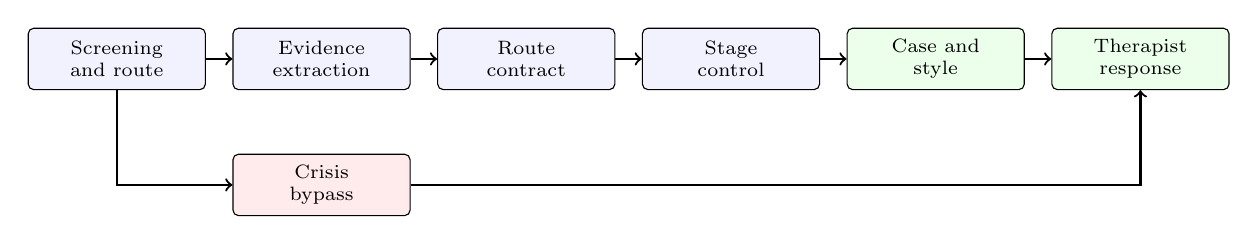
\begin{tikzpicture}[
  box/.style={draw, rounded corners=2pt, align=center, font=\scriptsize, minimum width=2.25cm, minimum height=0.78cm, fill=blue!5},
  plan/.style={draw, rounded corners=2pt, align=center, font=\scriptsize, minimum width=2.25cm, minimum height=0.78cm, fill=green!8},
  risk/.style={draw, rounded corners=2pt, align=center, font=\scriptsize, minimum width=2.25cm, minimum height=0.78cm, fill=red!8},
  arrow/.style={->, thick}
]
\node[box] (intake) at (0,0) {Screening\\and route};
\node[box] (evidence) at (2.6,0) {Evidence\\extraction};
\node[box] (contract) at (5.2,0) {Route\\contract};
\node[box] (stage) at (7.8,0) {Stage\\control};
\node[plan] (reasoning) at (10.4,0) {Case and\\style};
\node[plan] (response) at (13.0,0) {Therapist\\response};
\node[risk] (crisis) at (2.6,-1.6) {Crisis\\bypass};

\draw[arrow] (intake) -- (evidence);
\draw[arrow] (evidence) -- (contract);
\draw[arrow] (contract) -- (stage);
\draw[arrow] (stage) -- (reasoning);
\draw[arrow] (reasoning) -- (response);
\draw[arrow] (intake.south) |- (crisis.west);
\draw[arrow] (crisis.east) -| (response.south);
\end{tikzpicture}
\caption{Therapist core pipeline.}
\label{fig:therapist_core}
\end{figure}

\section{Blackboard Coordination}

\subsection{Shared State and Dialogue Graph}

The blackboard is the shared workspace of the system. It stores the current interpretation of the turn and the artifacts produced by each module. It is more than conversation history. It is a structured state that allows the assessor, peer agents, therapist, validator, safety layer, memory updater, and benchmark runner to coordinate without passing hidden instructions through natural language.

The dialogue graph organizes the execution order. A normal turn begins with onboarding or previous session context. The clinical assessor updates the blackboard. Nam and Linh observe the updated state and decide whether to draft a contribution. The therapist orchestrator reads the blackboard and peer drafts, creates the final message, and sends it through guardrails. The memory updater stores only visible messages.

This graph should not be interpreted as the therapist calling peer agents by command. Nam and Linh run as blackboard observers. Their execution means that they are allowed to look at the shared state, not that they are allowed to speak. Their draft remains internal until the therapist approves it.

\begin{table}[tb]
\centering
\caption{Main state groups in the blackboard.}
\label{tab:blackboard_state}
\scriptsize
\begin{tabular}{p{0.20\textwidth}p{0.36\textwidth}p{0.28\textwidth}}
\toprule
State group & Representative fields & Purpose \\
\midrule
Clinical state & \texttt{therapy\_route}, \texttt{previous\_stage}, \texttt{current\_stage}, \texttt{stage\_transition}, \texttt{stage\_confidence}, \texttt{stage\_evidence}, \texttt{stage\_goal} & Track route and stage interpretation \\
Evidence and formulation & \texttt{stage\_evidence\_details}, \texttt{case\_formulation} & Preserve observed signals and working hypothesis \\
Group state & \texttt{required\_yalom\_factors}, \texttt{peer\_drafts}, \texttt{peer\_contribution}\newline\texttt{\_decisions} & Control peer contribution and silence \\
Safety state & \texttt{safety\_flags}, \texttt{psychosocial\_safety}, \texttt{risk\_level} & Gate unsafe or boundary-risk output \\
Output state & \texttt{structured\_therapist\_plan}, \texttt{therapist\_validator}, \texttt{final\_output} & Deliver and audit final response \\
\bottomrule
\end{tabular}
\end{table}

\begin{figure}[tb]
\centering
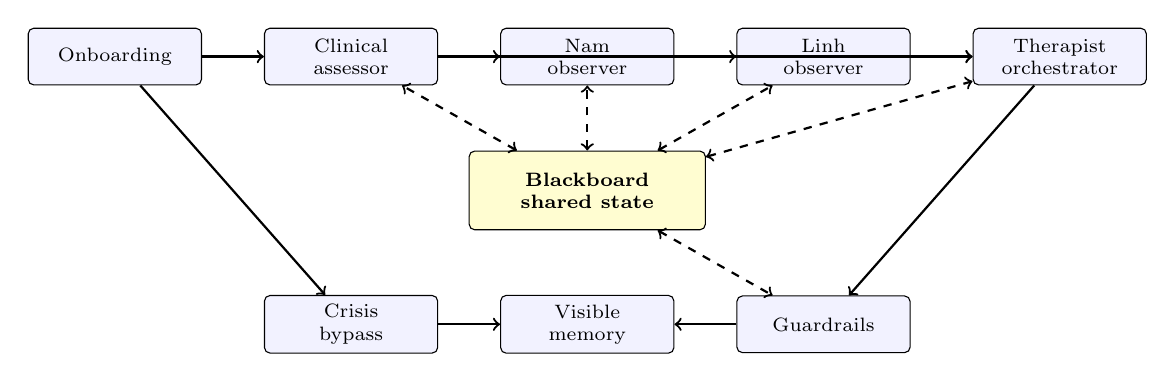
\begin{tikzpicture}[
  nodebox/.style={draw, rounded corners=2pt, align=center, font=\scriptsize, minimum width=2.2cm, minimum height=0.72cm, fill=blue!5},
  statebox/.style={draw, rounded corners=2pt, align=center, font=\scriptsize\bfseries, minimum width=3.0cm, minimum height=1.0cm, fill=yellow!18},
  arrow/.style={->, thick},
  readwrite/.style={<->, thick, dashed}
]
\node[statebox] (bb) at (6,0) {Blackboard\\shared state};
\node[nodebox] (onboard) at (0,1.7) {Onboarding};
\node[nodebox] (assess) at (3,1.7) {Clinical\\assessor};
\node[nodebox] (nam) at (6,1.7) {Nam\\observer};
\node[nodebox] (linh) at (9,1.7) {Linh\\observer};
\node[nodebox] (therapist) at (12,1.7) {Therapist\\orchestrator};
\node[nodebox] (guard) at (9,-1.7) {Guardrails};
\node[nodebox] (memory) at (6,-1.7) {Visible\\memory};
\node[nodebox] (crisis) at (3,-1.7) {Crisis\\bypass};

\draw[arrow] (onboard) -- (assess);
\draw[arrow] (assess) -- (nam);
\draw[arrow] (assess) -- (linh);
\draw[arrow] (nam) -- (therapist);
\draw[arrow] (linh) -- (therapist);
\draw[arrow] (therapist) -- (guard);
\draw[arrow] (guard) -- (memory);
\draw[arrow] (onboard) -- (crisis);
\draw[arrow] (crisis) -- (memory);
\draw[readwrite] (bb) -- (assess);
\draw[readwrite] (bb) -- (nam);
\draw[readwrite] (bb) -- (linh);
\draw[readwrite] (bb) -- (therapist);
\draw[readwrite] (bb) -- (guard);
\end{tikzpicture}
\caption{Blackboard coordination graph.}
\label{fig:blackboard_graph}
\end{figure}

\subsection{Output Assembly}

The final output is assembled only after therapist approval. If a peer draft is included, it is rendered as a separate speaker message such as Nam or Chị Linh. The therapist message is then rendered as Nhà trị liệu. This preserves the virtual group feeling while keeping the therapist as the organizing voice.

The orchestrator also checks for repetition between peer drafts and therapist speech. If the therapist response is too similar to an included peer draft, the system uses a bridge response or validator fallback to prevent the common failure where a peer speaks and the therapist immediately repeats the same sentence.

\subsection{Visible Memory and Internal Trace}

The memory updater stores only messages that the user actually sees. Discarded peer drafts, internal therapist plans, supervisor notes, and validator metadata may be kept for debugging and benchmark logs, but they are strictly excluded from the visible conversation history to ensure that later turns are not influenced by text the user never saw.

The internal trace remains valuable for evaluation. It records what the system believed, why it advanced or stayed in a stage, which peer drafts were considered, which validation checks passed, and whether a fallback was used. Chapter 4 uses this trace to support structural scoring and failure analysis.

\section{Peer Support Layer}

\subsection{Yalom-Inspired Peer Design}

The virtual group layer is added because one-to-one therapist support, even when strong, may not fully address isolation, shame, and hopelessness. A peer voice can help a user feel less alone or see that small recovery steps are possible. The system therefore uses a narrow subset of Yalom-inspired group factors rather than attempting to simulate full group psychotherapy \citep{Yalom2020GroupPsychotherapy}.

This layer is supportive, not directive. It should enrich the therapist response only when the current route, stage, safety state, and required Yalom factor make peer support appropriate. In other turns, silence is the correct behavior.

\subsubsection{Nam Peer Role}

Nam represents universality and catharsis. His role is emotional mirroring and shame reduction. A valid Nam contribution is short, grounded in the user's feeling, and non-directive. Nam should help the user sense that their experience is understandable and not uniquely shameful.

Nam must not perform CBT, ask technical questions, give advice, name cognitive distortions, or lead the session. If he starts to act like a therapist, the persona validator rejects the draft or the therapist discards it.

\subsubsection{Linh Peer Role}

Linh represents hope and interpersonal learning. Her role is to offer brief realistic hope or a limited lived-experience perspective when the user expresses discouragement, hopelessness, or uncertainty about recovery. Linh's contribution should be short and should return attention to the user's next small step.

Linh must not overpromise, use toxic positivity, tell a long personal story, or instruct the user with phrases such as ``you should'' or ``you must''. Her value comes from realistic witness, not from advice.

\begin{table}[tb]
\centering
\caption{Peer role contract.}
\label{tab:peer_roles}
\small
\begin{tabular}{p{0.14\textwidth}p{0.24\textwidth}p{0.34\textwidth}p{0.16\textwidth}}
\toprule
Agent & Function & Allowed behavior & Must avoid \\
\midrule
Nam & Universality and catharsis & Short emotional reflection, normalization, shame reduction & Advice and CBT technique \\
Linh & Hope and interpersonal learning & Short realistic hope or lived-experience witness & Toxic positivity and long story \\
Therapist & Final clinical voice & Include, rewrite, or discard peer drafts & Mechanical repetition \\
\bottomrule
\end{tabular}
\end{table}

\subsection{Contribution Control}

\subsubsection{Contribution and Silence}

Each peer reads the blackboard and returns either a draft or a no-contribution decision. A draft records sender, contribution type, therapeutic function, Yalom factor, text, reason, confidence, and safety risk. A no-contribution decision is not a failure. It is a useful signal that the peer recognized the current stage does not need their function.

Silence is especially important in CBT Socratic questioning, acute MBI grounding, and safety cases. A peer story can interrupt guided discovery, distract from grounding, or soften a necessary safety boundary. The system therefore treats silence as an explicit peer skill.

\subsubsection{Persona Validation}

Peer outputs are checked against role and stage rules before they can appear. The validator rejects wrong-peer usage, advice, role drift, long self-disclosure, therapist-like technique, toxic positivity, and contributions in stages where peer speech should be silent. This gives Nam and Linh distinct identities instead of letting them become smaller versions of the therapist.

\begin{table}[tb]
\centering
\caption{Peer contribution and silence policy.}
\label{tab:peer_decision_rules}
\small
\begin{tabular}{p{0.36\textwidth}p{0.22\textwidth}p{0.28\textwidth}}
\toprule
Condition & Decision & Reason \\
\midrule
High safety risk is present & \texttt{NO\_CONTRIBUTION} & Safety response must remain therapist-led \\
Required Yalom factor does not match peer role & \texttt{NO\_CONTRIBUTION} & Prevent irrelevant peer messages \\
Current stage forbids peer interruption & \texttt{NO\_CONTRIBUTION} & Preserve CBT/MBI/BA technique fidelity \\
Draft gives advice, steals technique, or repeats therapist & Reject or discard & Prevent role drift and redundancy \\
Yalom factor, stage, persona, and safety all match & Draft may be used & Add controlled group support \\
\bottomrule
\end{tabular}
\end{table}

\subsubsection{Therapist Approval}

Peer drafts are never sent directly to the user. The therapist decides whether to include, rewrite, or discard each draft. If a draft is emotionally useful but too long or slightly off-role, the therapist can rewrite it. If it conflicts with stage, safety, or the therapist plan, it is discarded.

\begin{figure}[tb]
\centering
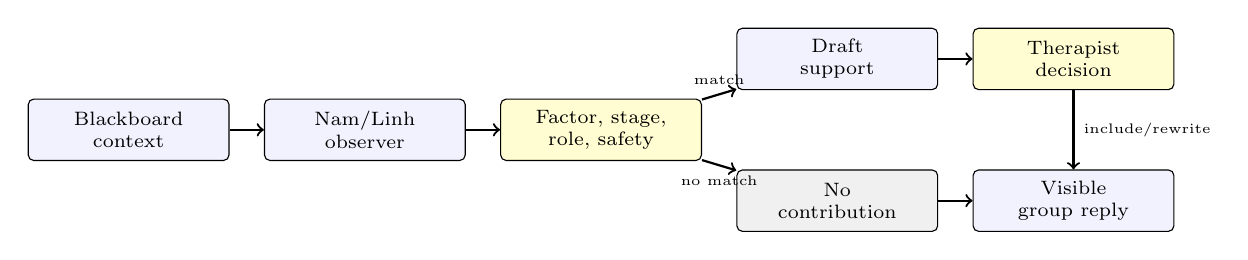
\begin{tikzpicture}[
  box/.style={draw, rounded corners=2pt, align=center, font=\scriptsize, minimum width=2.55cm, minimum height=0.78cm, fill=blue!5},
  decision/.style={draw, rounded corners=2pt, align=center, font=\scriptsize, minimum width=2.55cm, minimum height=0.78cm, fill=yellow!18},
  stopbox/.style={draw, rounded corners=2pt, align=center, font=\scriptsize, minimum width=2.55cm, minimum height=0.78cm, fill=gray!12},
  arrow/.style={->, thick}
]
\node[box] (bb) at (0,0) {Blackboard\\context};
\node[box] (peer) at (3.0,0) {Nam/Linh\\observer};
\node[decision] (check) at (6.0,0) {Factor, stage,\\role, safety};
\node[box] (draft) at (9.0,0.9) {Draft\\support};
\node[stopbox] (silent) at (9.0,-0.9) {No\\contribution};
\node[decision] (therapist) at (12.0,0.9) {Therapist\\decision};
\node[box] (visible) at (12.0,-0.9) {Visible\\group reply};

\draw[arrow] (bb) -- (peer);
\draw[arrow] (peer) -- (check);
\draw[arrow] (check) -- node[above, font=\tiny]{match} (draft);
\draw[arrow] (check) -- node[below, font=\tiny]{no match} (silent);
\draw[arrow] (draft) -- (therapist);
\draw[arrow] (therapist) -- node[right, font=\tiny]{include/rewrite} (visible);
\draw[arrow] (silent.east) -- (visible.west);
\end{tikzpicture}
\caption{Peer contribution decision flow.}
\label{fig:peer_support_flow}
\end{figure}

\section{Safety and Evaluation Trace}

\subsection{Validation and Supervisor Audit}

\subsubsection{Response Validation}

The response validator checks whether the therapist output fits the current route and stage. CBT Stage 1 should validate emotion and invite context. CBT Stage 3 should gently name a cognitive pattern. CBT Stage 4 should ask an evidence-oriented or double-standard Socratic question. MBI responses should not debate the truth of thoughts during grounding. BA responses should keep actions small enough for the user's energy level.

The validator returns a validity result, reason, optional fallback, and quality scores such as stage fit, specificity, empathy, focus, and safety. If the generated response violates the route contract, the validator can replace it with a safer stage-specific fallback. This mechanism turns many generation failures into inspectable repairs.

\subsubsection{Supervisor Audit}

The supervisor audit is a diagnostic layer after response generation. It checks whether the route is locked, the stage is present, the technique is valid, peer usage follows route and Yalom policy, and safety flags do not indicate high-risk output. Such a diagnostic layer is essential because a response can sound fluent while still violating the system contract; the audit notes make these violations much easier to trace.

\begin{table}[tb]
\centering
\caption{Supervisor audit checks.}
\label{tab:supervisor_audit}
\small
\begin{tabular}{p{0.24\textwidth}p{0.42\textwidth}p{0.20\textwidth}}
\toprule
Audit item & Question answered & Failure signal \\
\midrule
Route lock & Is the response still inside CBT, MBI, BA, or crisis handling? & Route drift \\
Stage lock & Does the response know the active stage? & Missing stage state \\
Technique validity & Does the therapist response satisfy the route contract? & Wrong technique \\
Peer use validity & Are Nam/Linh allowed for this route, stage, and factor? & Wrong peer or unwanted peer \\
Safety validity & Do safety critics or flags show unsafe output risk? & Rewrite or fallback needed \\
\bottomrule
\end{tabular}
\end{table}

\subsection{Psychosocial Safety}
\label{sec:psychosocial_safety}

\subsubsection{Safety Critics}

The safety layer checks more than explicit crisis language. It reviews user input, peer drafts, therapist speech, and the combined output for psychosocial risks. The current critics cover crisis, medical boundary, dependency, manipulation or over-agreement, and privacy or bias. Evaluating these aspects is crucial because mental-health systems can fail through subtle relational harms rather than just obvious unsafe advice \citep{Li2025CounselBench,Luo2025DialogGuard}.

\begin{table}[tb]
\centering
\caption{Safety critics and fallback actions.}
\label{tab:safety_critics}
\small
\begin{tabular}{p{0.20\textwidth}p{0.30\textwidth}p{0.16\textwidth}p{0.20\textwidth}}
\toprule
Critic & Example risk & Severity & Action \\
\midrule
Crisis & Self-harm, violence, abuse, immediate danger & High & Bypass peers and use crisis-safe response \\
Medical boundary & Diagnosis, medication dosage, clinical decision request & Medium/High & Redirect to professional care \\
Dependency & User treats chatbot as only support & Medium & Encourage real-world support and autonomy \\
Manipulation & Over-agreement, coercion, harmful reassurance & Medium & Rewrite or fallback \\
Privacy and bias & Excessive personal data or discriminatory framing & Low/Medium & Remove unsafe framing and minimize data collection \\
\bottomrule
\end{tabular}
\end{table}

\subsubsection{Crisis Bypass}

When the input contains acute safety risk, the system does not continue ordinary therapy routing. The graph bypasses peer observers and produces a direct safety-focused therapist response. The response avoids therapeutic exploration and instead prioritizes immediate safety, real-world support, and emergency contact when appropriate.

The crisis bypass is intentionally conservative. In a supportive research prototype, missing a high-risk signal is more serious than pausing an ordinary route too early. For this reason, high-risk safety state overrides peer support, route progression, and ordinary stage work.

\subsection{Benchmark Logs}

Every turn can produce a benchmark trace: route, previous stage, current stage, FSM transition, confidence, evidence, case formulation, required Yalom factors, peer decisions, therapist plan, validator result, safety critics, final output, and fallback use. Serving as a primary implementation artifact for Chapter 4, the trace allows the system to be measured at the level of therapeutic behavior rather than relying solely on final text quality.

Furthermore, relying on this metadata supports a fairer evaluation process. The proposed system exposes internal metadata for structural checks, while external baselines are evaluated from visible response text. Chapter 4 therefore separates deterministic metadata scoring, text-based judging, human audit, confidence intervals, and failure taxonomy.

\begin{figure}[tb]
\centering
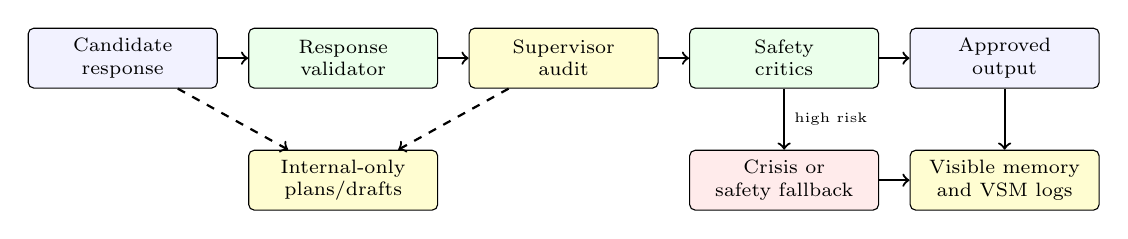
\begin{tikzpicture}[
  box/.style={draw, rounded corners=2pt, align=center, font=\scriptsize, minimum width=2.4cm, minimum height=0.76cm, fill=blue!5},
  check/.style={draw, rounded corners=2pt, align=center, font=\scriptsize, minimum width=2.4cm, minimum height=0.76cm, fill=green!8},
  risk/.style={draw, rounded corners=2pt, align=center, font=\scriptsize, minimum width=2.4cm, minimum height=0.76cm, fill=red!8},
  trace/.style={draw, rounded corners=2pt, align=center, font=\scriptsize, minimum width=2.4cm, minimum height=0.76cm, fill=yellow!18},
  arrow/.style={->, thick}
]
\node[box] (candidate) at (0,0) {Candidate\\response};
\node[check] (validator) at (2.8,0) {Response\\validator};
\node[trace] (audit) at (5.6,0) {Supervisor\\audit};
\node[check] (safety) at (8.4,0) {Safety\\critics};
\node[box] (approved) at (11.2,0) {Approved\\output};
\node[trace] (logs) at (11.2,-1.55) {Visible memory\\and VSM logs};
\node[risk] (fallback) at (8.4,-1.55) {Crisis or\\safety fallback};
\node[trace] (internal) at (2.8,-1.55) {Internal-only\\plans/drafts};

\draw[arrow] (candidate) -- (validator);
\draw[arrow] (validator) -- (audit);
\draw[arrow] (audit) -- (safety);
\draw[arrow] (safety) -- (approved);
\draw[arrow] (approved) -- (logs);
\draw[arrow] (safety) -- node[right, font=\tiny]{high risk} (fallback);
\draw[arrow] (fallback) -- (logs);
\draw[arrow, dashed] (candidate) -- (internal);
\draw[arrow, dashed] (audit) -- (internal);
\end{tikzpicture}
\caption{Safety and benchmark trace pipeline.}
\label{fig:safety_trace}
\end{figure}

Overall, Chapter 3 translates the research gaps from Chapter 2 into a working system design. The therapist core provides guided therapeutic progression, the blackboard keeps all components aligned, the peer layer creates a limited virtual group presence, and the safety trace makes the response process inspectable. These design choices are evaluated in Chapter 4 through multi-turn benchmark cases and failure analysis.
